\chapter{Wireless Communication and Network Embedded Systems}

\section{Embedded Systems}
With internet of things (IoT) we have \adef{sensors} that we get data from and 
then we an \adef{actuator} component to control a mechanism or system.

%real-time requirements
%TinyOS: Allows manymodule concurrent activities to be serviced on a single stack
%Contiki: Multi-threading: One stack per thread
% protothread: Multi-threading on a single stack
%Contiki Protothreads allows conditional blocking wait PROCESS_WAIT_UNTIL(c). Wait for event, will be put to bocking.
%This macro is similar to PROCESS_WAIT_EVENT() in that it blocks the currently running process until the process receives an event. But PROCESS_WAIT_EVENT_UNTIL() takes an extra condition which must be true for the process to continue.

\begin{definitionblock}{Blocking Calls}
    When a thread asks the kernel to do something that doesn't require executing instructions,
    like reading a sensors value or receiving a packet from the network. 
    The thread will then be put in a wait queue for when the operation completes.
\end{definitionblock}

\begin{definitionblock}{Asynchronous Calls}
    Thread makes a call to start an operation and will not block, i.e. call will return.
    The read can later check if operation is complete using polling or block on wait()>
\end{definitionblock}



\subsection{TinyOS}
TinyOS is used for sensor network and a very low foot print.

Key features and design principles of TinyOS
\begin{itemize}
    \item Work schedular and many drivers for microcontrollers and ICs.
    \item Resource use minimization, in form of computational efficient, little stat (RAM), tight code (ROM), and motivated by energy and cost.
    \item Bug prevention: It does not allow recursion, constraints preclude extensive logging. Static, compile-time operations.
    It has extensive logging. Memory allocation predictable.
    \item Event driven approach meaning instead of creating threads that does specific tasks we react on events instead through interrupt.
    Which does not make sense when the embedded system is continually running.
    \item tasks perform primary work. Atomic, run to completion, deferred procedure call.
    That is whe it is possible to allocate a single stack.
    \item Split-phase: is when a \adef{command} request to initiate some action  and the \adef{event} represent completion of a request or something.
    \item System modularity: named component and interfaces which consists of command and event, see Figure~\ref{fig:tinyos_component_model}.
    \item TinyOS no system/user boundary nor system services.
    \item Does not allow preemption, is instead but in a FIFO queue. 
\end{itemize}

%Event-driven concurrency
%since it only runs a single command?

\begin{figure}[H]
    \centering
    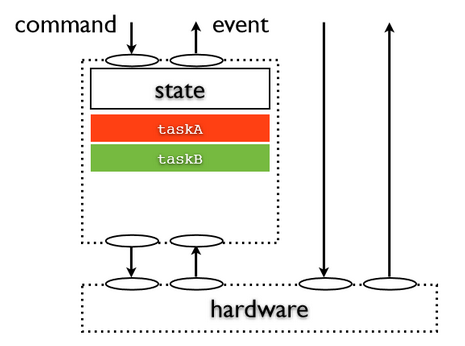
\includegraphics[width=10cm]{\imagesPath/tinyos_component_model.png}
    \caption{TinyOS component model.}
    \label{fig:tinyos_component_model}
\end{figure}

Programing av TinyOS with nearly c \textit{*.nc} is done with first defining the \adef{module configuration}
then the \adef{Module Implementation}. 


%Active message???
%Single Hop communication????


\subsection{Contiki}
\begin{itemize}
    \item cooperative: runs sequentially with respect to other cooperative code.
    \item preemtive: temporarily stops the cooperative code
\end{itemize}

There are \adef{asynchronous events}, \adef{synchronous events}. 

Contiki multi-threading 
\begin{itemize}
    \item Combining event-driven and threads : Multithreading those applications that needs it.
    \item Protothread, multi-threading on a single stack, which make it light-weight.
\end{itemize}

Power down when there are no events scheduled.

\begin{figure}[H]
    \centering
    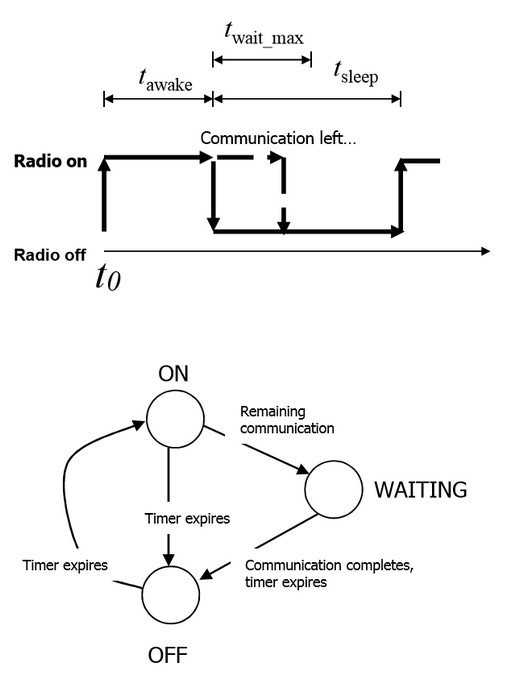
\includegraphics[width=10cm]{\imagesPath/hypothetical_mac_protocol.png}
    \caption{If there is no incoming message within $t_{awake}$ then quit else resive until maximum or when resived. }
    \label{fig:Hypothetical MAC Protocol}
\end{figure}

Nullnet, buffer there is blocking in contiki, don't know how.
TinyOS is only event-driven contiki allows for events but there are also threads, it uses protothread.

PROCESS\_WAIT\_EVENT\_UNTIL(c) puts the thread into a waiting queue
and will be put in ready queue after the interrupt occurs.
%https://dak664.github.io/contiki-doxygen/a01627.html#_details 


\subsection{Intermittent computing}
\adef{Intermittent computing} where the power is frequently lost and regained.
Often does not have batteries or just small ones. Instead they can use capacitors and some energy harvesting methods like solar panel.
This issue is handled by taking \adef{checkpoints}, where the program is in a certain state so that it can continue when power is back up again.

\begin{figure}[H]
    \centering
    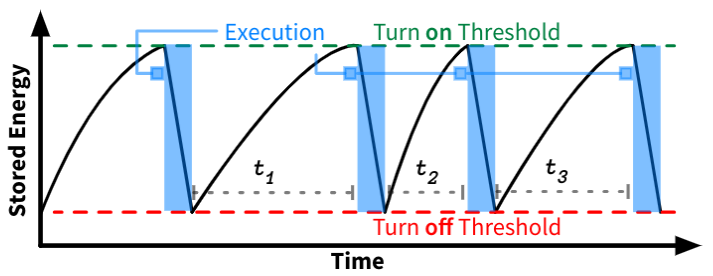
\includegraphics[width=10cm]{\imagesPath/intermittent_power.png}
    \caption{Intermittent power}
    \label{fig:intermittent_power}
\end{figure}


\section{Wireless Communication}

\subsection{Radio Communication}
\begin{figure}[H]
    \centering
    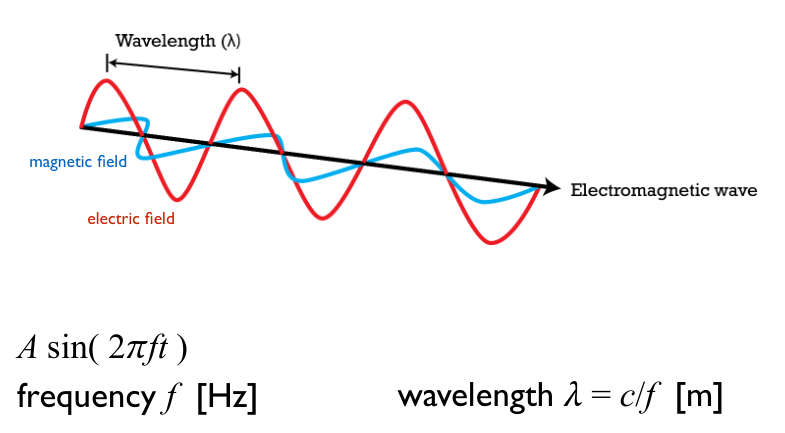
\includegraphics[width=10cm]{\imagesPath/electromagnetic_waves.png}
    \caption{Electromagnetic waves. We can assume that c, the speed of light, is $3*10^8$}
\end{figure}

\begin{figure}[H]
    \centering
    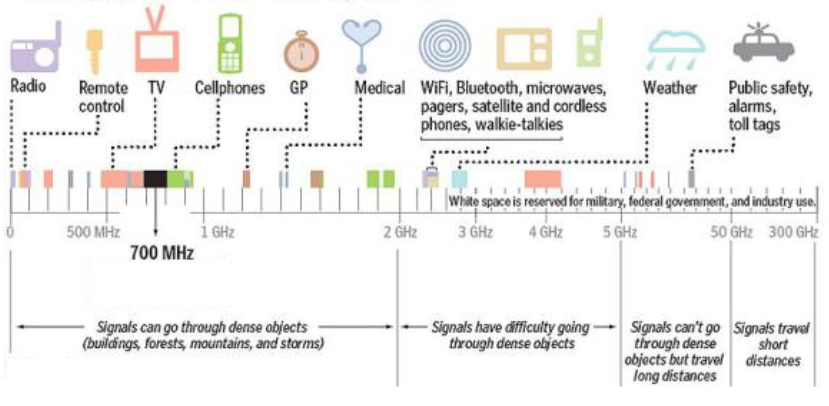
\includegraphics[width=10cm]{\imagesPath/frequency_spectrum.png}
    \caption{Radio frequency spectrum.}
\end{figure}

Industrial, Scientific, Medical Band (ISM) is License free. The other bands 
are allocated by the government and some purchased by companies and organization 
in the public sector.

\adef{Propagation}: the behavior of radio waves as the travel.

\begin{figure}[H]
    \centering
    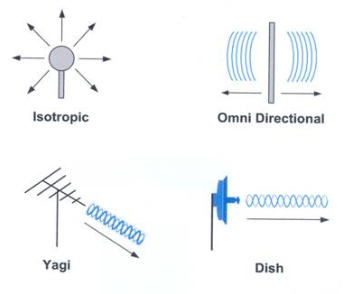
\includegraphics[width=10cm]{\imagesPath/antenna_types.png}
    \caption{Antenna types.}
\end{figure}

\begin{figure}[H]
    \centering
    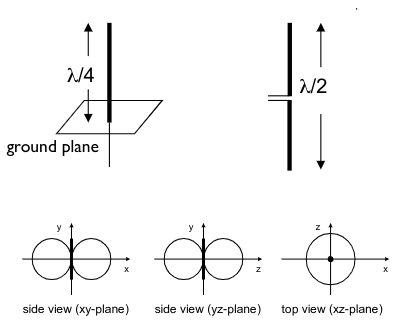
\includegraphics[width=10cm]{\imagesPath/monopole_dipole_antenna.png}
    \caption{Monopole/dipole antenna.}
\end{figure}

Isotrpoic radiator will form a sphere thus the power of the signal is:
\begin{equation}
    P_u = P_{Tx}A_u/A_s = P_{Tx}/4\pi r^2,
\end{equation}
since the area of a sphere $A_s=4\pi r^2$ and area of a unit are $A_u = 1$.
$P_Tx$ is the power of the transmitted signal. Thus $P_u$ decreases whit the square of the distance.

The size of the antenna matters as it can receive more of the signal.
It is called Aperture, which for receiver (Rx) antenna can be calculated as: 
\begin{equation}
    A = G\frac{\lambda^2}{4\pi},
\end{equation}
where $G$ is the antenna gain and $\lambda$ is the wavelength.
Antenna gain is how efficient the antenna is the higher the gain.
Thus, the gain for isotropic is less then with a dish antenna.
The key take away is that the received signals become waker with higher frequency.

Radiated power received at the antenna:
\begin{equation}
    P_{Rx} = P_uA = P_{Tx}G_{Tx}G_{Rx}\left( \frac{\lambda}{4\pi r} \right)^2,
\end{equation}
The higher the frequency the shorter the wavelength and thus the lower the received power.

Decibel power ratio between the transmit power and and the antennas type reference power.
\begin{equation}
    L_P = 10\log_{10}\frac{P}{P_0}dB
\end{equation}
reference to $P_0 = 1 mW$.

\adef{Free-Space Path Loss} is the attenuation (gradual loss) of radio energy 
from the transmitting antenna and the receiving antenna.
\begin{equation}
    FSPL = \frac{P_{Tx}}{P_{Rx}} = \left( \frac{4\pi r}{\lambda} \right)^2
\end{equation}
When increasing the wavelength we decrease the path loss.

\adef{Two-eay ground propagation model}: how reflection of the ground affect the strength of the receiver. 
\begin{figure}[H]
    \centering
    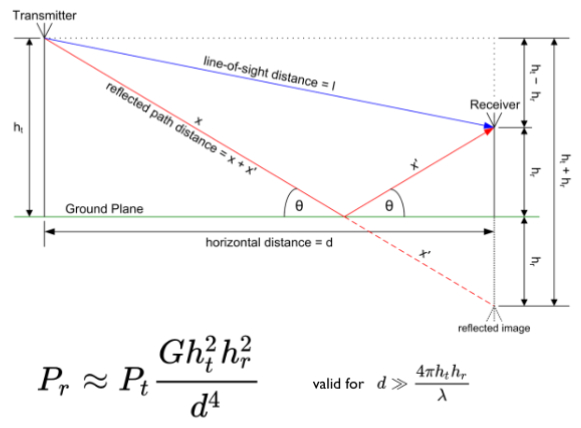
\includegraphics[width=10cm]{\imagesPath/two-eay_ground_propagation_model.png}
    \caption{Two-eay ground propagation model.}
\end{figure}

Two-ray ground propagation model formula:
\begin{equation}
    PL = P_{t_{dBm}} - P_{r_{dBm}} = 40\log_{10}(d) - 10\log_{10}(Gh^2_th^2_r)
\end{equation}
The higher the antenna the lower the path loss.


\begin{definitionblock}{COST Hata Propogation Model}
    A model that has been created from experiments and observation, thus it can not be derived.

    \begin{equation}
        L = 46.3 + 33.9\log{f} - 13.82\log{h_B} - a(h_R,f) + [44.9 - 6.55\log{h_B}]\log{d} + C
    \end{equation}

    For suburban or rural environments:
    \begin{equation}
        a(h_R,f) = (1.1\log{F} - 0.7)h_R - (1.56\log{f} - 0.8)
    \end{equation}

    For large cities:
    \begin{equation}
        a(h_R,f) = 
        \begin{cases} 
            8.29 ( \log_{10}(1.54h_R))^2 - 1.1, \; \text{if} 150 \leq f \leq 200 \\
            3.2 ( \log_{10}(11.75h_R))^2 - 4.97, \; \text{if} 200 \leq f \leq 1500
        \end{cases} 
    \end{equation}

    \begin{equation}
        C =
        \begin{cases} 
            0 dB \text{ for medium cities and suburban areas} 
            3 dB \text{ for metropolitan areas} 
        \end{cases} 
    \end{equation}

    \begin{itemize}
        \item $L$ = Median path loss, Unit: decibel (dB)
        \item $f$ = Frequency of Transmission. Unit: megahertz (MHz)
        \item $h_B$ = Base station antenna effective height. Unit: meter (m)
        \item $d$ = Link distance. Unit: Kilometer (km)
        \item $h_R$ = Mobile station antenna effective height. Unit: meter (m)
        \item $a(h_R)$ = Mobile station antenna heght correction factor as described in the Hata model for urban areas.
    \end{itemize}
\end{definitionblock}

\begin{figure}[H]
    \centering
    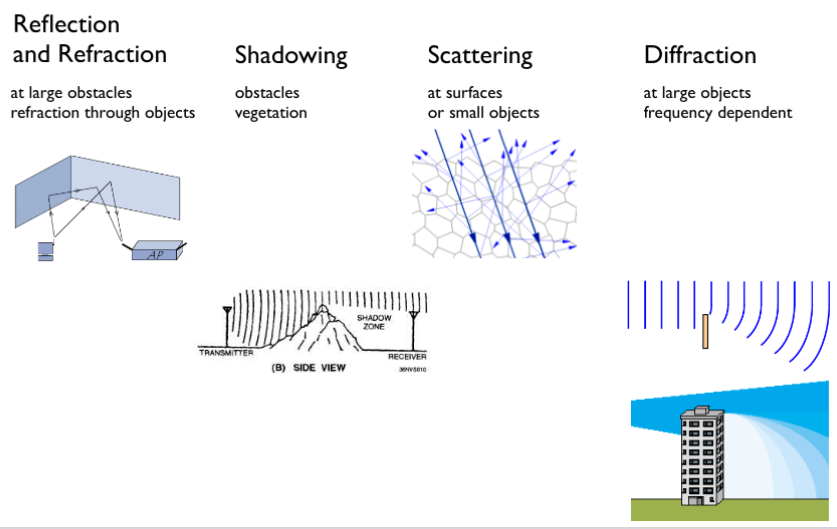
\includegraphics[width=10cm]{\imagesPath/propagation.png}
    \caption{Propagation. Reflection and refraction refers how waves changes direction in contact with materials. Note that waves phase change by $\pi$ at reflection.
    Shadowing refers to obstacle that blocks the signals from the receiver.
    Scattering refers to signals scatter in a an object, can be due to material which is very un even.
    Diffraction refers to how signals changes there wavefront by moving threw tight objects or openings.}
\end{figure}

\adef{Multi-Path Progagation}: signals can often take multiple paths to arrive at the receiver which could result in a distorted received signal 
as the received signal is the combination of all of the paths the signal took to arrive at the receiver.

\adef{Fading} when two signals cancel each other out. There can occurs something called \adef{deep fade} 
were in that spot the signal is not noticeable. This can be fixed by moving the receiver or transmitter.

Embedded antennas
\begin{itemize}
    \item PCB antenna, peak gain 3.5 dBi
    \item SMD antenna (eg BLE,WiFi), peak gain 2.1 dBi
\end{itemize}

\adef{Link Budget} is the how the signal strength decreases over time and we need to make sure 
it is above the budget or a threshold.

\begin{figure}[H]
    \centering
    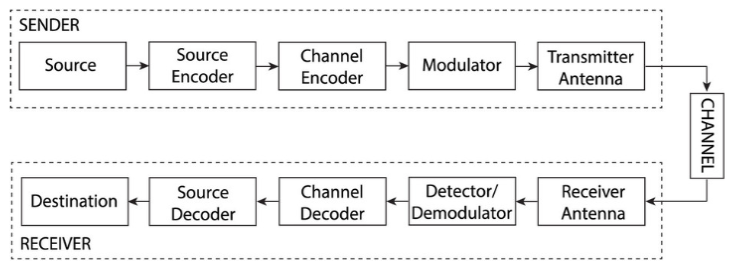
\includegraphics[width=10cm]{\imagesPath/wireless_systems.png}
    \caption{Wireless systems from source to destination.}
\end{figure}


\subsubsection{Analog Modulation}
\begin{align}
    x(t) &= \textcolor{red}{A(t)}\sin(2\pi \textcolor{red}{f(t)}t + \textcolor{red}{\varphi(t)}) \\
    s(t) &= x(t)\cdot\sin(2\pi f_c t)
\end{align}

\begin{figure}[H]
    \centering
    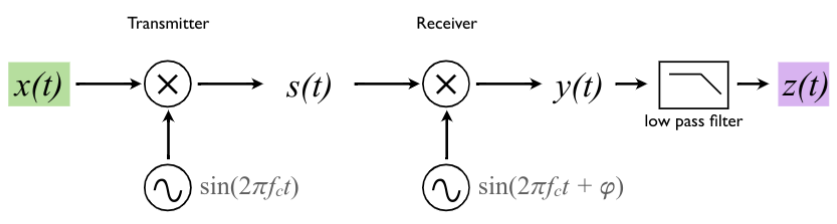
\includegraphics[width=10cm]{\imagesPath/analog_modulation.png}
    \caption{Analog Modulation}
\end{figure}

\subsection{Digital Modulation}
To represent a bit sequence we can use a modulation order of 2 or more
\begin{itemize}
    \item 1 bit, $\{0,1\} \to M = 2$ symbols
    \item 2 bit, $\{00,01,10,11\} \to M = 4$ symbols
    \item \ldots
    \item k bits, $M = 2^k$ symbols
\end{itemize}

\begin{equation}
    S(t) = \textcolor{red}{A(t)}\cos[2\pi \textcolor{red}{f(t)}t + \textcolor{red}{\varphi(t)}] \\
\end{equation}

Modulation schemes
\begin{itemize}
    \item ASK, amplitude shift keying, have diffrent amplitudes to represent diffrent symbols
    \item FSK, frequency shift keying.
    \item PSK, phase shift keying.
    \item QAM, change both phase and amplitude.
\end{itemize}

When sending out a signal it must be within a certain frequency band.
\adef{Passband signal}.
\begin{align}
    S_P(t) &= a(t)\cos[2\pi f_c t + \phi(t) ] \\
           &= \textcolor{blue}{a(t)\cos(\phi(t))}\cos(2\pi f_c t) - \textcolor{orange}{a(t)\sin(\phi(t))}\sin(2\pi f_c t) \\
           &= \textcolor{blue}{S_I(t)}\cos(2\pi f_c t) - \textcolor{orange}{S_Q}\sin(2\pi f_c t)
\end{align}
The sin and cos terms are octagonal, so they do not interfere with one another.
$S_I$ and $S_Q$ defines the coordinates of the symbol.

\adef{Constellation diagram} shows the symbols in a complex plan. The real axis is called \adef{in-phase} and the 
imaginary access is called \adef{quadratic}.


\subsection{Error and loss}
\adef{Symbol error rate} is how often a symbol is interpreted as another symbol.
\adef{Bit error rate} is how many bits are wrong, this could be more than symbol energy since each 
symbol can contain more than one bit and depending on if it is binary bitmap or gray bitmap it could be 
a higher probability that there is a >1 bit error.
\adef{Packet error rate} is the rate of which a packets was unsuccessfully received.
If a single bit in a packet is wrong it could lead to the whole package becomes unusable.

\adef{Additive white Gaussian noise (AWGN)} applies noise to the input so the output has some disturbance.

\adef{Signal-to-noise ratio (SNR)}:
\begin{equation}
    SNR = \frac{E_S}{N_0}
\end{equation}

\begin{figure}[H]
    \centering
    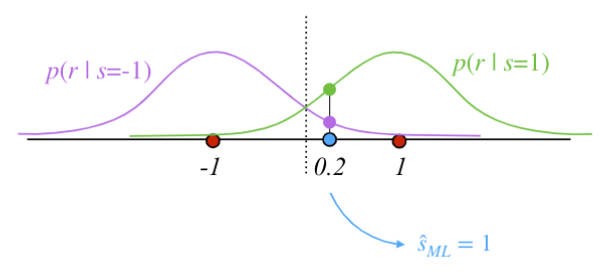
\includegraphics[width=10cm]{\imagesPath/maximum_likelihood.png}
    \caption{Maximum likelihood (ML) decision}
\end{figure}

Performance
\begin{itemize}
    \item speed $\rightarrow$ high \adef{bit rate}
    \item reliability $\rightarrow$ low \adef{bit error rate} (BER)
    \item energy efficiency $\rightarrow$ low \adef{energy per bit} ($E_b$) to \adef{noise power} ($N_0$) ratio.
\end{itemize}

\begin{equation}
    \textit{Bit rate} = \textit{symbol rate} \times \log_2(M)
\end{equation}
M is the modulation order.

\begin{figure}[H]
    \centering
    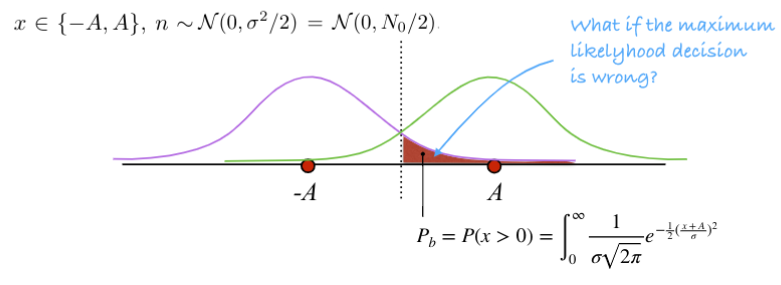
\includegraphics[width=10cm]{\imagesPath/symbol_error_pobability.png}
    \caption{Reliability: Symbol Error Probability (BPSK)}
\end{figure}

Remember Bayes' theorem.
\begin{equation}
    p(s|r) = \frac{p(r|s)p(s)}{p(r)}
\end{equation}

%%%%%%%%%%%%%%%%%%%%%%%%%%%%%%%%%%%%%%%%%%%%%%%%%%%%%%%%%%%%%
%%%%%%%%%%%%%%%%%%%%%%%% BEGIN DONT UNDERSTAND %%%%%%%%%%%%%%
%%%%%%%%%%%%%%%%%%%%%%%%%%%%%%%%%%%%%%%%%%%%%%%%%%%%%%%%%%%%%

MAP rule (M modulation order):
\begin{align*}
    \hat{s}_{MAP} &= \arg\max_{s_i} p(s_i|r) \\
                  &= \arg\max_{s_i} p(r|s_i)p(s_i) \\
\end{align*}

\begin{definitionblock}{Q-Function} 
    For a standard Gaussian random variable, $X ~ N(0,1)$, the Q-function  
    Q(x) gives the probability of $X>x$:
    \begin{equation}
        Q(x)  P (X>x)
    \end{equation}
    For non-standard Gaussian random variable, $Y~N(\mu, \sigma^2)$:
    \begin{equation}
        P(Y>y) = Q(\frac{y-\mu}{\sigma})
    \end{equation}
\end{definitionblock}


\begin{definitionblock}{Calculating the Error Probability (BPSK)}
    Energy per symbol: $E_s = \frac{1}{M}\sum_{i=1}^{M} ||s_i||^2$

    Energy per bit: $E_b = \frac{E_s}{\log_2(M)}$

    $P_e(\hat{s}_{ML}) = Q\left( \sqrt{\frac{2E_b}{N_0}} \right)$
\end{definitionblock}


\begin{exampleblock}{Signal Power}
    \begin{equation*}
        s(t) = A\sin(2\pi f_0 t)
    \end{equation*}

    \begin{align*}
        P &= \frac{1}{T_0} \int_{-T_0/2}^{T_0/2} (A\sin(2\pi f_0t))^2 dt \\
          &= \frac{1}{T_0} \int_{0}^{T_0/2} A^2\frac{1-\cos(4\pi f_0t)}{2} dt \\
          &= \frac{1}{T_0} \left[ A^2t - \frac{A^2}{4\pi f_0}\sin(4\pi f_0 t) dt \right]_{t=0}^{t={T_0/2}} \\
          &= \frac{A^2}{2}
    \end{align*}
\end{exampleblock}


\begin{exampleblock}{Symbol Energy}
    ASK with points $1/4$, $1/2$, $3/4$, $1$.

    Average energy per symbol
    \begin{equation*}
        E_s = \frac{1}{M}\sum_{i=1}^M \left[ \frac{A^2}{2} \right]
    \end{equation*}

    \begin{align*}
        E_s &= \frac{1}{4} \left[ 
             \frac{1}{2}\left(\frac{1}{4}\right)^2 
            +\frac{1}{2}\left(\frac{3}{4}\right)^2 
            +\frac{1}{2}1^2 \right] T_s \\
            &= \frac{1}{8} \left[ \frac{1}{16} + \frac{1}{4} + \frac{9}{16} + 1\right]
            = \frac{30}{8\times 16}T_s
    \end{align*}
\end{exampleblock}


%%%%%%%%%%%%%%%%%%%%%%%%%%%%%%%%%%%%%%%%%%%%%%%%%%%%%%%%%%%%%
%%%%%%%%%%%%%%%%%%%%%%%% END DON'T UNDERSTAND %%%%%%%%%%%%%%%
%%%%%%%%%%%%%%%%%%%%%%%%%%%%%%%%%%%%%%%%%%%%%%%%%%%%%%%%%%%%%

\begin{definitionblock}{This is called Shannon-Hartley Channel Capacity}
    The capacity of the channel in respect to bandwidth $B$ and 
    Signal to Noise Ration $SNR$:
    \begin{equation}
        C = B\log_2(1+SNR)
    \end{equation}
    Due to nykvist theorem $f_s>2B$ therefore we can send samples up to $f_s\leq2B$
    SNR $M=1+\frac{A}{\delta{V}}$, $M=\sqrt{1+SNR}$. B is the with of the frequency allowed.
\end{definitionblock}

\adef{Packet Errors} to handle errors we can use:
\begin{itemize}
    \item ARQ schemes: using acknowledgments (ACK) to confirm reception.
    \begin{itemize}
        \item Negative ACK (NACK) or (NAK) is sent to indicate that there were som kind of error with the received package.
        \item Cumulative ACK is an acknowledgments for successfully received packages, the ack includes the number of frames.
    \end{itemize}
    \item Error Correction Coding: add redundancy to the data to recover errors at the receiver.
    \begin{itemize}
        \item Forward Error Correcting (FEC). 
    \end{itemize}
\end{itemize}

Packet Error Rate.
\begin{equation}
    PER = 1 - (1-BER)^l
\end{equation}

\begin{align*}
    ETX = E[transmission] &= \sum_{k=0}^{\infty} p(k)k = \sum_{k=0}^{\infty} (1-p)p^{k-1}k \\
                          &= \frac{1-p}{p}\sum_{k=0}^{\infty} p(k)k = \frac{1-p}{p}\frac{p}{(1-p)^2} \\
\end{align*}
\begin{equation}
    ETX = \frac{1}{1-p}
\end{equation}

\begin{figure}[H]
    \centering
    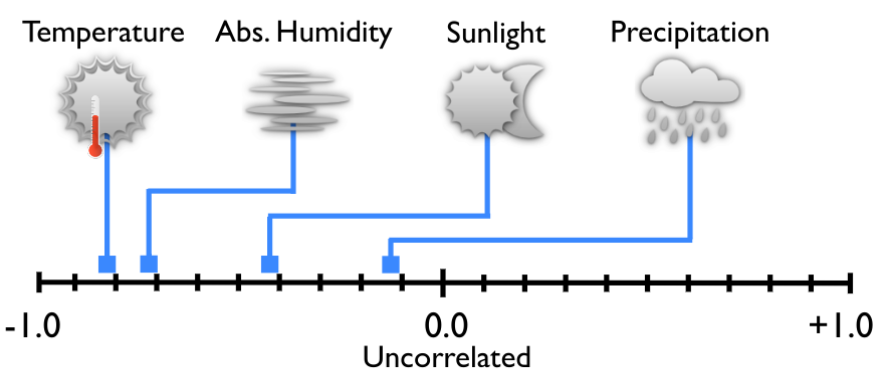
\includegraphics[width=10cm]{\imagesPath/meteorological_impact.png}
    \caption{Meteorological Impact}
\end{figure}

Relaying, send a package to an intermittent node to later pass it on the the destination node.
Spanning Tree are used to show how many message are sent. 
When we want to get results from all nodes using relaying we could eather 
combined the result before passing it on or not. 
This is called \adef{aggregation} and when we use it the number of message are 
the number of nodes. Without aggregation the $\sum_{depth=1}^{max_{depth}} depth*nodes_{depth}$
\begin{align*}
    \sum_i d_in_i \text{w/o aggregation} \\
    \sum_i n_i\text{with aggregation} \\
\end{align*}


\subsection{Medium Access}
\begin{figure}[H]
    \centering
    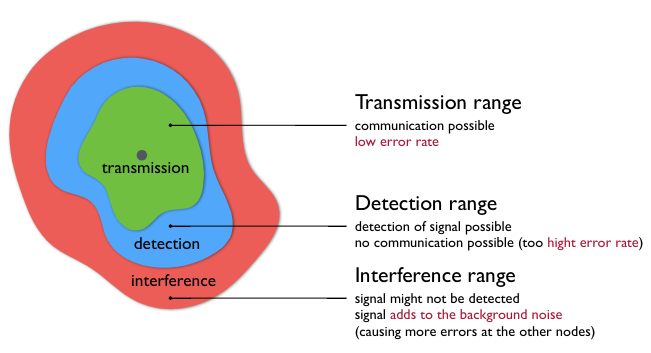
\includegraphics[width=10cm]{\imagesPath/medium_access.png}
    \caption{Medium access}
\end{figure}

Signal to Noise plus Interference Ratio:
\begin{equation}
    SNIR = \frac{S}{N+I}
\end{equation}
where $S$ is the signal energy, $N$ is the noise energy, and $I$ is the interference energy.

\adef{Collisions} if we receive multiple frames at the same time.
To prevent this we need to coordinate the access of multiple senders.
This problem is called \adef{Multiple Access Problem}.

There are different protocols \adef{Multiple access protocol}.
\begin{center}
\begin{tabular}{ |m{4cm}|m{1.2cm}|m{1.5cm}|m{1cm}|m{2.5cm}|m{1cm}|m{1cm}| } 
     \hline
                                                           & TDMA       & FDMA         & SDMA        & TDMA/FDMA & CDMA & CSMA \\ 
     \hline
     only one node transmitting: throughput of R bits/s    & In timeskt & No           & if only one & ?         & No   & Yes  \\ 
     \hline
     N nodes have data: each has throughput R/N in average & Yes        & Yes          & No          & Yes       & Yes  & No   \\ 
     \hline
     decentralized                                         & Yes        & Probably not & Yes         & ?         & Yes  & Yes  \\
     \hline
     simple                                                & ?          & ?            & Yes         & ?         & ?    & Yes  \\
     \hline
\end{tabular}
\end{center}

Channel Partioning protocols: TDMA, FDMA, CDMA (time, frequency, code)
Random Access protocols: Aloha, CSMA, CSMA/CD

\subsubsection{Time Division Multiplexing}
\begin{figure}[H]
    \centering
    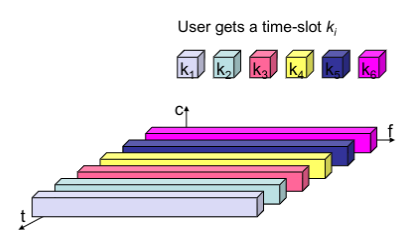
\includegraphics[width=10cm]{\imagesPath/tdma.png}
    \caption{TDMA: A user gets the whole allocated band for an given timeslot $t$}
\end{figure}

\subsubsection{Frequency Division Multiplexing}
\begin{figure}[H]
    \centering
    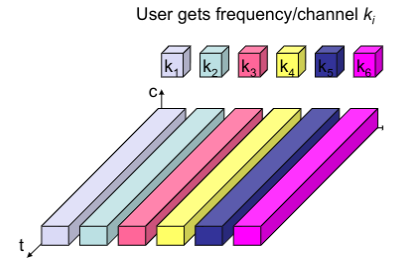
\includegraphics[width=10cm]{\imagesPath/fdma.png}
    \caption{FDMA: A user have a certain frequency band.}
\end{figure}

\subsubsection{Space Division Multiplexing}
\begin{figure}[H]
    \centering
    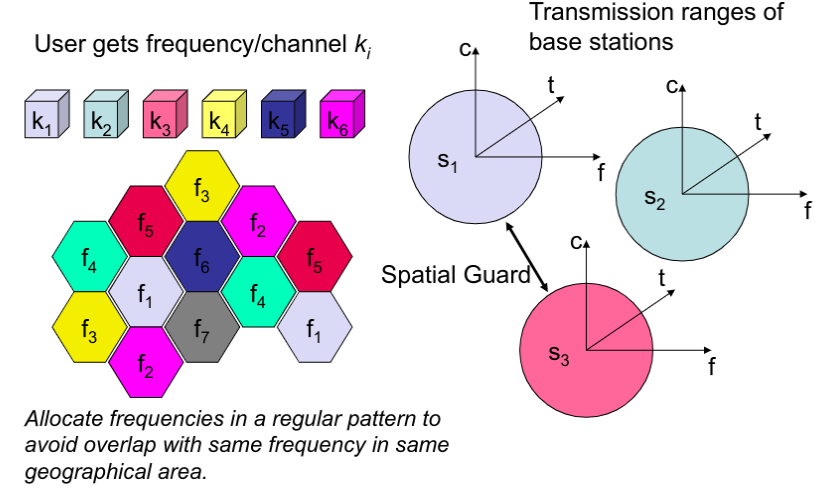
\includegraphics[width=10cm]{\imagesPath/sdma.png}
    \caption{SDMA: Allocates frequencies in regular patterns so that it avoid overlap with the same frequency in the same geograpical area.
    It can be thought of only sending the signal to a specific geographical area.}
\end{figure}

\subsubsection{Code Division Multiplexing}
\begin{figure}[H]
    \centering
    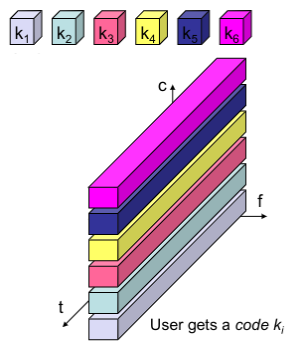
\includegraphics[width=6cm]{\imagesPath/cdma.png}
    \caption{CDMA: Each user uses ave access to the whole frequency band and can use all available time.
    There will, however, be a specific code that each user has and the codes are octagonal from each other, thus not cousing interference.}
\end{figure}

\begin{figure}[H]
    \centering
    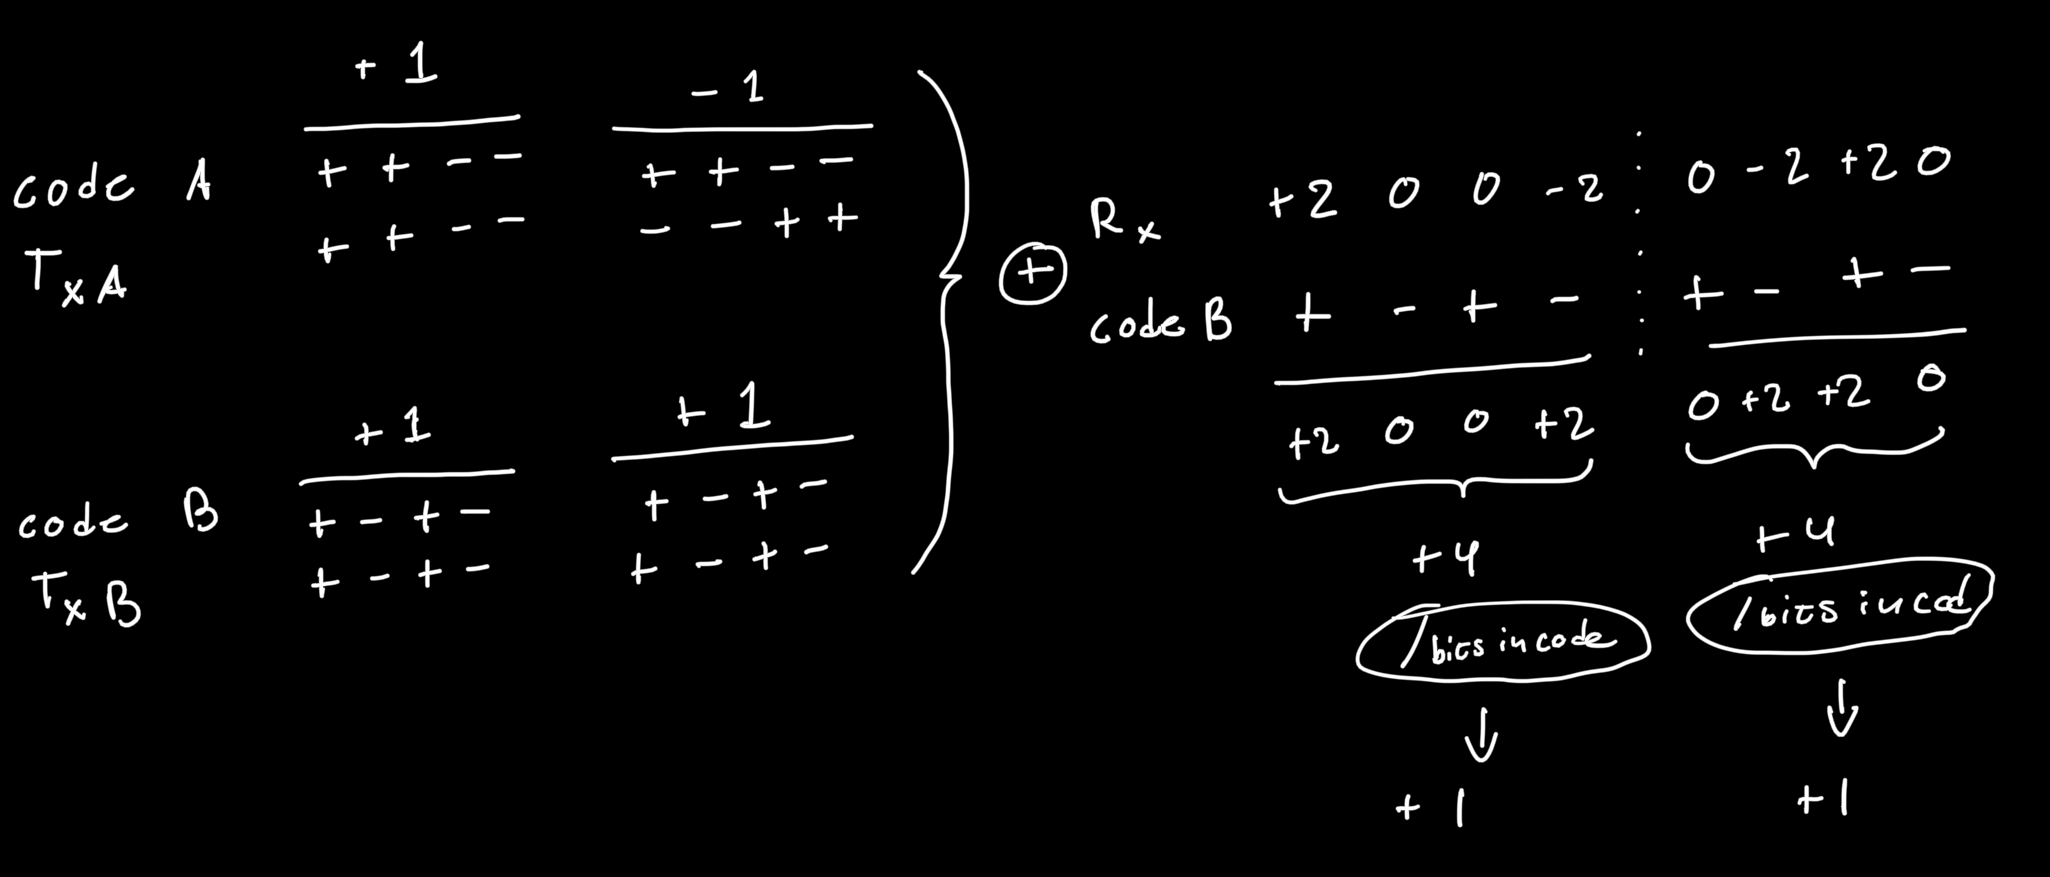
\includegraphics[width=12cm]{\imagesPath/cdma_code.png}
    \caption{CDMA decode and encode.}
\end{figure}


\subsection{CSMA/CD in Wireless Network}
\begin{figure}[H]
    \centering
    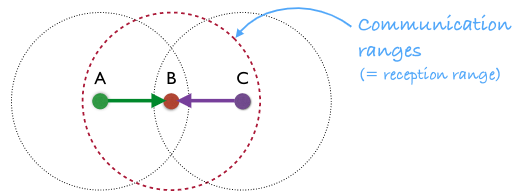
\includegraphics[width=10cm]{\imagesPath/hidden_terminal_problem.png}
    \caption{Hidden Node Problem or Hidden terminal problem. C cannot know that A is sending to B and not detect collision.}
\end{figure}

To solve hidden terminal problem we first send out an \adef{Request to Send (RTS)}. Then 
when the destination node (B) has received it it will send out a \adef{Clear to Send (CTS)} 
to both A and C. If C has received only a CTS and not a RTS then it knows there might be collisions.
Then B will send an ack that is has been received which will also give a C the go to send a RTS.

\begin{figure}[H]
    \centering
    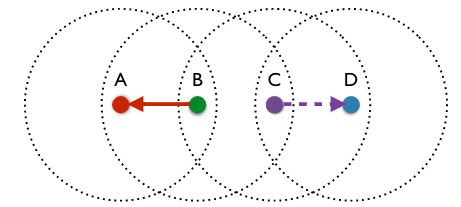
\includegraphics[width=10cm]{\imagesPath/exposed_terminal_problem.png}
    \caption{Exposed Node Problem or Exposed terminal problem. The problem is that C is prevented to send to D when B wants to send to A.}
\end{figure}

To solve exposed node problem B first sends out a RTS and then A will answer with a CTS. 
C will ignore the RTS since it does not want to send to A, thus C can send to D.

\begin{figure}[H]
    \centering
    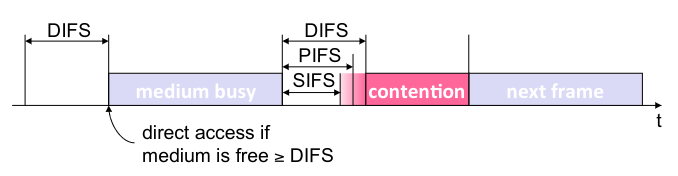
\includegraphics[width=10cm]{\imagesPath/collision_avoidance.png}
    \caption{Collision avoidance (CSMA/CA). The sender wights DIFS-time to sense disturbance in channel. 
    The receiver wights SIFS-time to send the ACK.}
\end{figure}

\begin{figure}[H]
    \centering
    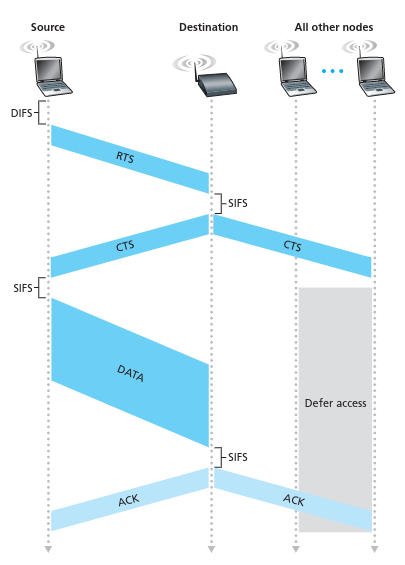
\includegraphics[width=10cm]{\imagesPath/rts-cts.png}
    \caption{WiFi 802.11 with RTS/CTS.}
\end{figure}

%https://www.youtube.com/watch?v=3F4DQINyx3g


\section{Networked Embedded Systems}

\subsection{IoT}
The internet of things, be it sensors or devices, that collect data and may be 
remotely controlled over the internet.

\adef{Sensors} are things that measure and \adef{actuators} are things that 
control or do something physical like a smart lamp.

Privacy
\begin{itemize}
    \item Anonymize data
    \item Use of aggregated data instead of individual data points
    \item Operate on encrypted data (e.g., homomorphic cryptography)
    \item add noise to the data (e.g., location privacy)
\end{itemize}

Application models
\begin{itemize}
    \item Application logic on the small devices
    \begin{itemize}
        \item Low latency
        \item More privacy (no guarantee)
        \item Avoid communication cost
    \end{itemize}
    \item Application logic in the cloud
    \begin{itemize}
        \item More powerful applications combining data from many devices and sources
        \item sensor data sent to the cloud
    \end{itemize}
\end{itemize}

IoT using different communication protocols.
\begin{itemize}
    \item Internet Protocol (IP)
    \begin{itemize}
        \item The pervasive nature of IP networks allows use of existing infrastructure
        \item IP-based technologies already exist, are well-known, and proven to be working.
        \item Open and freely available specifications vd closed proprietary solutions.
        \item IP-based devices can be connected readily to other IP-based networks, without the need for intermediate entities like translation gateways or proxies.
    \end{itemize}
    \item Lightweight internet protocol
    \begin{itemize}
        \item Fragmentation, Header Compression. Header compression can be done on \textit{common values}, \textit{duplicate information that can be derived from other layers}, and \textit{shared context}.
    \end{itemize}
    \item Non-internet protocols, like ZigBee. Reduces the overhead that will be cursed by internet protocol.
\end{itemize}